\section{Marco teórico}

Para el desarrollo de este trabajo se abordan temas como la obtención de datos (visión por computadora), clasificación (RANSAC) y la implementación de AGC.  Por lo cual, a continuación, se describen los conceptos necesarios para el desarrollo.

\subsection{Representación Digital}

Una imagen digital es guardada según el formato de imagen (TIFF, BMP, JPEG, etc.), pero todas las imágenes luego de su interpretación son representadas en una computadora por un arreglo bidimensional de \glspl{pixel}.\\

El arreglo de píxeles se puede ver como un conjunto de matrices numéricas, dependiendo la representación del píxel (RGB, CMY, RGBA, CMYA, etc.) son los canales necesarios para representarlo por completo. Así una imagen en RGB (rojo, verde, azul por sus siglas en inglés) cuenta con tres canales, cada canal define la intensidad de cada color, así para mostrar una imagen $MxN$ en RGB es necesario tres matrices de $M$ filas y $N$ columnas.\\

De esta manera es posible generar una imagen nueva a partir de otras realizando operaciones sobre imágenes como la suma, resta y multiplicación, aplicando una transformación como se muestra en la ecuación \eqref[ec.]{eq:transfimg}.\\

\begin{equation}
\label{eq:transfimg}
q(x,y)=f(p_1(x,y),p_2(x,y))
\end{equation}
Donde $p_1$ es un píxel de la imagen 1 y $p_2$ un píxel de la imagen 2 y $q(x,y)$ el píxel resultante de la nueva imagen \cite{martinsanz2007ejercicios}.\\

Una \gls{nube de puntos} se describe como el conjunto de puntos en un espacio dado o una estructura de datos usada para representar una colección de puntos \cite{weinmann2016reconstruction}. Al trabajar con nubes de puntos se pueden pensar en ellas como una imagen de tres dimensiones y en lugar de un píxel se trabajan sobre \glspl{punto}. Al igual que las imágenes.\\

A diferencia de una \gls{imagen} una nube de puntos puede o no estar organizada en filas y columnas, sensores como el Kinect en los que se obtiene una imagen de profundidad se obtiene una nube de puntos de $MxN$ puntos, mientras que otras nubes de puntos tienden a ser solo una lista $Mx1$ de puntos en el espacio \cite{Rusu_ICRA2011_PCL}.\\


\subsection{Sensor Kinect}

En el desarrollo de vídeo juegos, la competencia entre grandes empresas ha dado como resultado en una variedad de dispositivos que le permiten al usuario una interacción más natural con entornos virtuales. Estos dispositivos son variados tanto en sus componentes físicos como en la forma de interacción. unos de los dispositivos más conocidos son el Wii Mote, PS/Move y el Kinect.\\

Para la consola Wii de Nintendo se usa un Wii Mote, mostrado en la figura \ref{fig:WiiMote}, que, con el uso de una barra de leds infrarrojos y sensores de posición y aceleración, es capaz de obtener su posición respecto la barra de leds \cite{UsodelKi56:online}.\\
\begin{figure}[!htb]
	\centering
	\includegraphics[width=0.4\textwidth]{01Introduccion/imagenes/wiiMote.JPG}
	\caption{Control Wii Mote de Nintendo} 
	\label{fig:WiiMote}
\end{figure}


En el caso del PlayStation de Sony, que usa un PS/Move, mostrado en la figura \ref{fig:psMove}, se usa una cámara de vídeo que, junto con sensores de posición y aceleración, se realiza esta interacción.\\

\begin{figure}[!htb]
	\centering
	\includegraphics[width=0.2\textwidth]{01Introduccion/imagenes/PsMOve.JPG}
	\caption{Control PS/Move de Sony} 
	\label{fig:psMove}
\end{figure}

Mientras que Xbox de Microsoft optó por un dispositivo realizado por la empresa PrimeSense llamado Kinect, el cual integra micrófonos, un motor, un emisor infrarrojo, una cámara de vídeo a color y otra infrarroja \cite{UsodelKi56:online}, el dispositivo se muestra en la figura \ref{fig:kinect1} \cite{Microsof29:online}. Usando la cámara infrarroja el Kinect detecta la profundidad de objetos usando una técnica llamada tiempo de vuelo (Time of Flight ToF), en la cual se obtiene el tiempo que tarda un rayo de luz en rebotar en un objeto, sabiendo la velocidad del rayo de luz y el tiempo desde su emisión hasta que es captado por la cámara, se calcula la distancia del objeto al sensor\cite{Lachat2015}.\\

\begin{figure}[!htb]
	\centering
	\includegraphics[width=0.7\textwidth]{01Introduccion/imagenes/xbox360kinect.JPG}
	\caption{Sensor Kinect 1} 
	\label{fig:kinect1}
\end{figure}

El dispositivo Kinect cuenta con dos versiones el primero se anunció con la consola Xbox 360 en el 2010 y el Kinect 2.0, mostrado en la figura \ref{fig:kinect}, se anunció junto a la Xbox One en 2013 los cuales cuentan con las características mostradas en la tabla \ref{tab:Kinect} \cite{UsodelKi56:online}.\\

% Please add the following required packages to your document preamble:
% \usepackage{graphicx}
\begin{table}[!htb]
	\centering
	\caption{Tabla comparativa de los modelos del Kinect}
	\label{tab:Kinect}
	\begin{tabular}{lll}
		\hline
		Característica                    & Kinect 1          & Kinect 2            \\ \hline
		Cámara de color                   & 640 x 480 @30 fps & 1920 x 1080 @30 fps \\
		Cámara de profundidad             & 320 x 240         & 512 x 424           \\
		Profundidad Máxima                & $\sim$4.5 m       & $\sim$4.5 m         \\
		Distancia de profundidad mínima   & 40 cm             & 50 cm               \\
		Visión de campo horizontal        & 57 grados         & 70 grados           \\
		Visión de campo vertical          & 43 grados         & 60 grados           \\
		Motor de inclinación              & si                & no                  \\
		Uniones definidas para esqueletos & 20 uniones        & 26 uniones          \\
		Esqueletos rastreados             & 2                 & 6                   \\
		Estándar USB                      & 2.0               & 3.0                 \\ \hline
	\end{tabular}%
\end{table}

\begin{figure}[!htb]
	\centering
	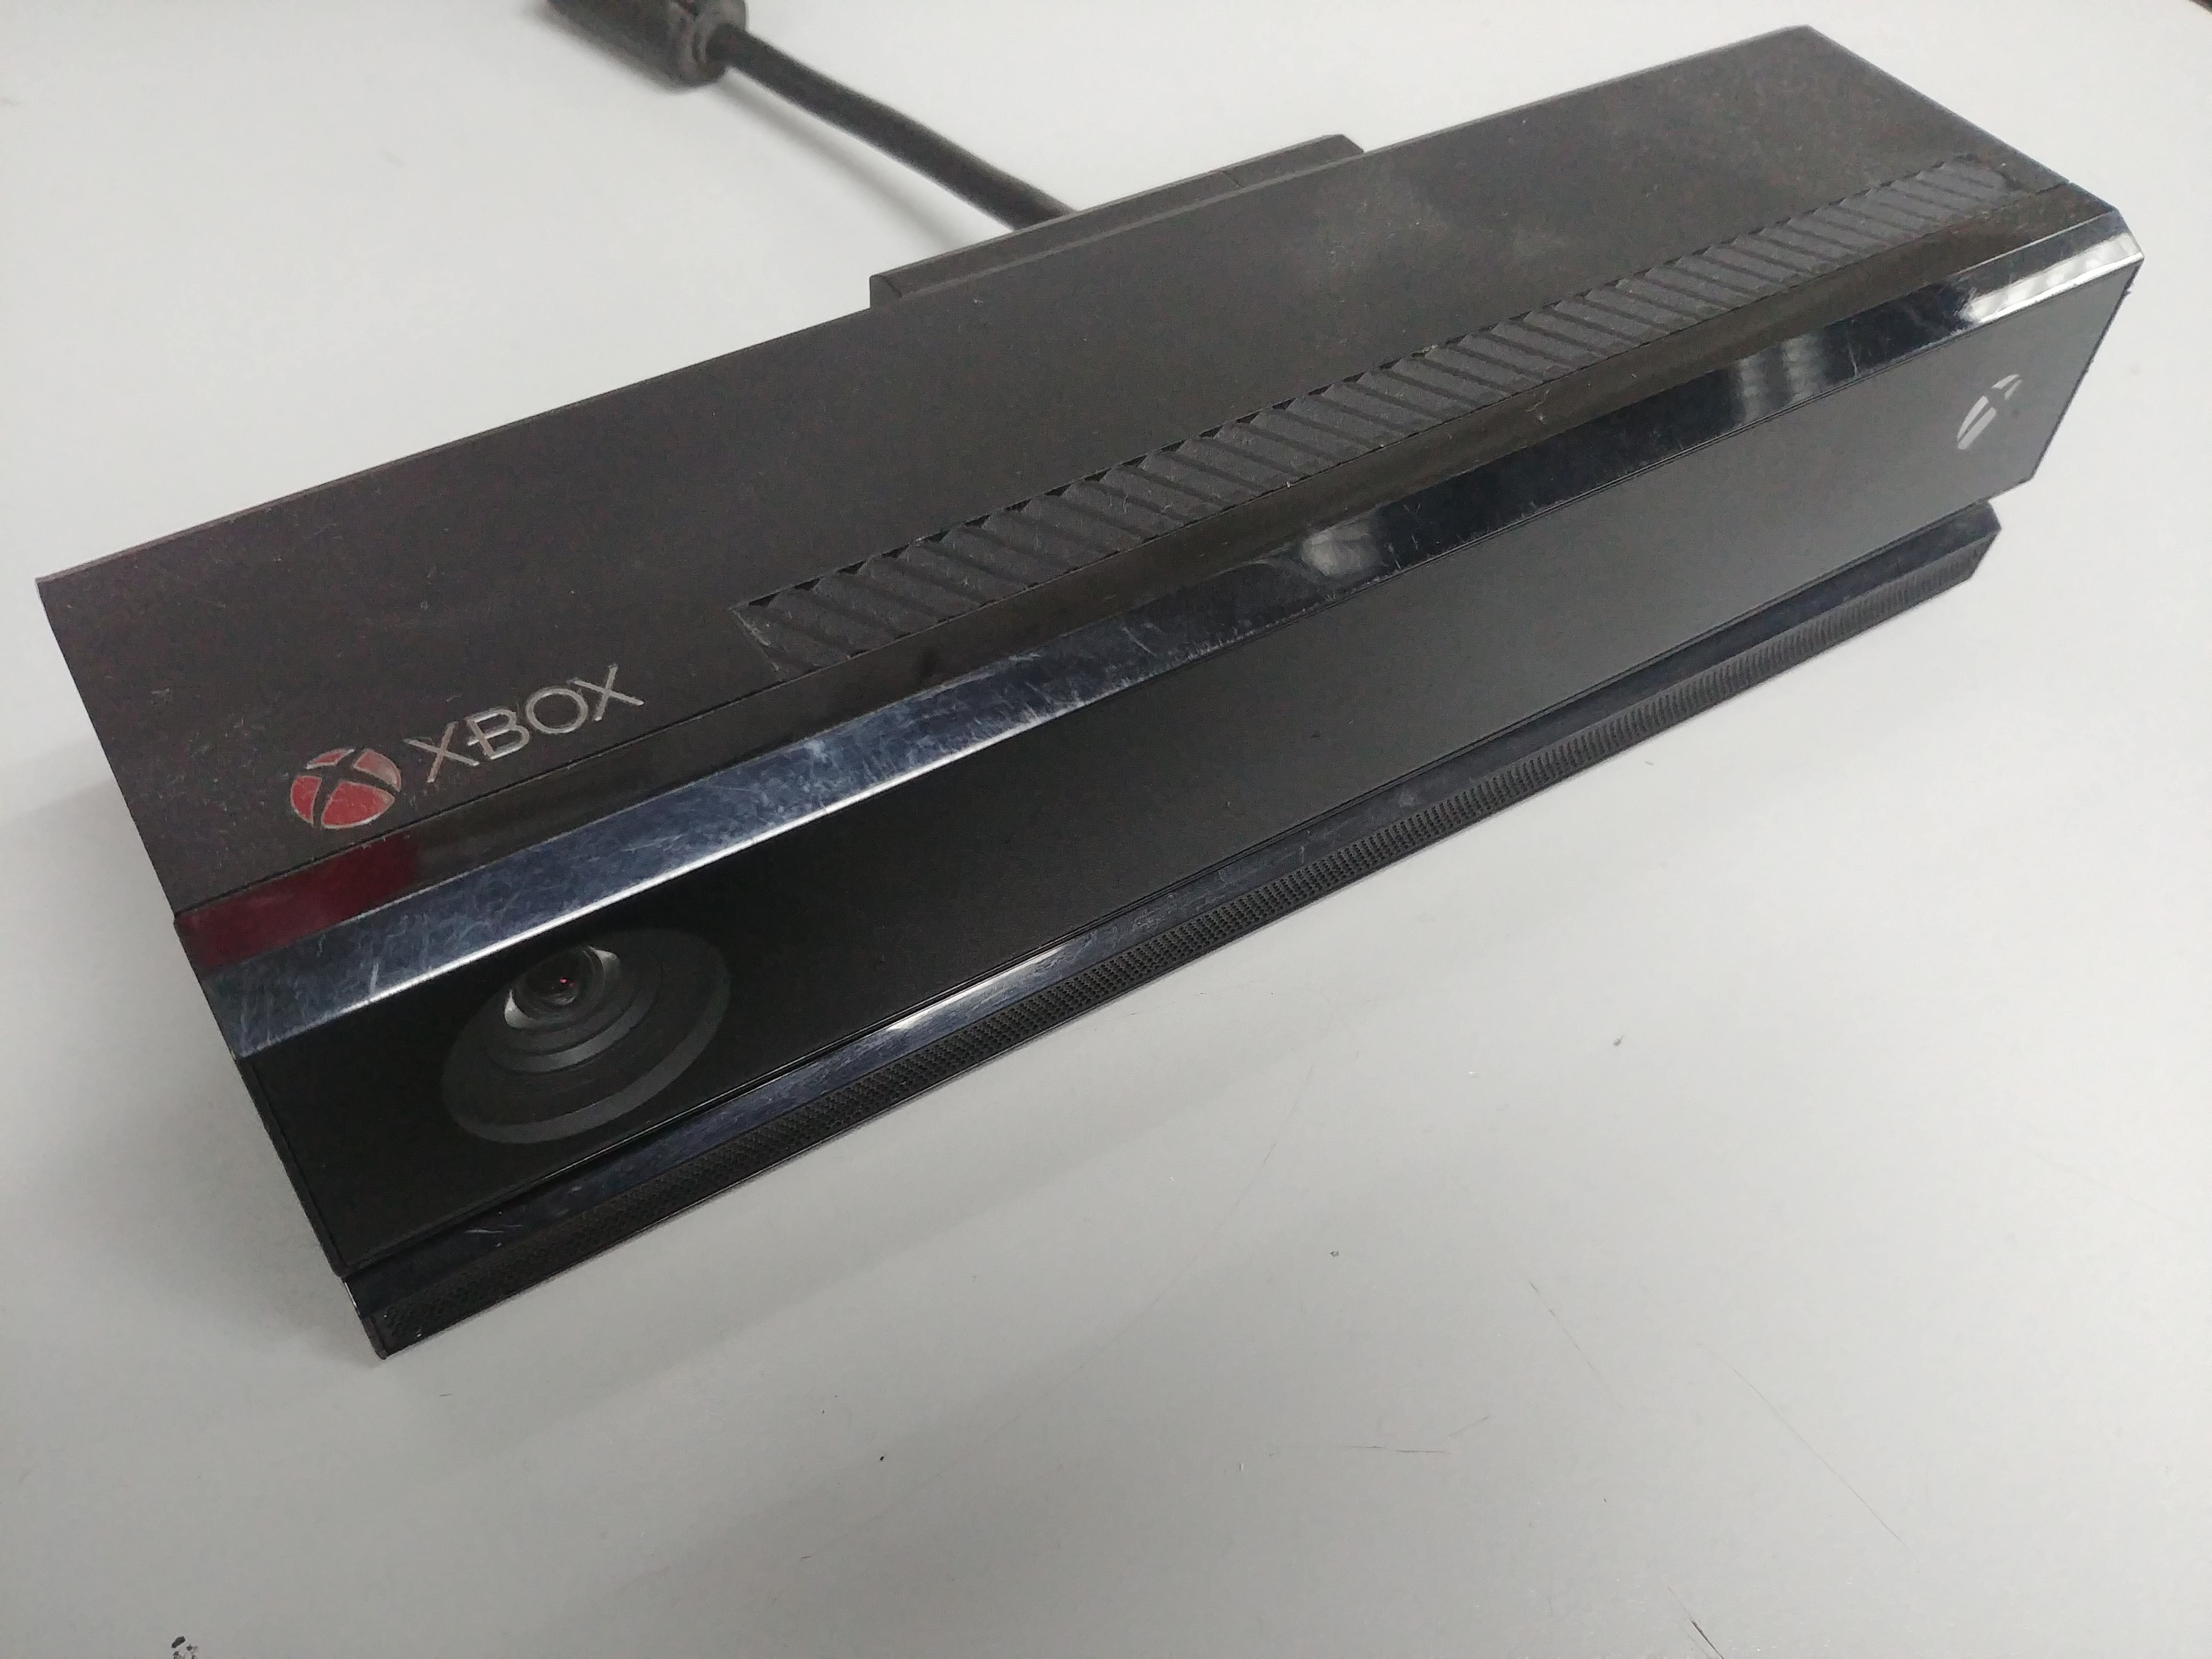
\includegraphics[width=0.6\textwidth]{02Desarrollo/Preprocesamiento/imagenes/20181017_182538[1].jpg}
	\caption{Sensor Kinect 2.0} 
	\label{fig:kinect}
\end{figure}



\subsection{Visión Por Computadora}

La visión por computadora trata de describir el mundo que vemos a partir de una o varias imágenes y reconstruir sus propiedades, como forma, color e intensidad de luz, tratando de imitar la visión de una persona. Es usada en gran cantidad de aplicaciones como: reconocimiento óptico de letras, inspección de productos en fábricas, modelado 3D, reconocimiento facial, etc. \cite{CompVisionSpringer}.\\

Se llevan a cabo varios procesos antes de someter una imagen a reconocimiento, esto sirve para resaltar puntos importantes, facilitar la detección de características, eliminar ruido, etc. Estos procesos son diferentes según el problema a tratar, pero ayudan en gran medida mejorar el reconocimiento de objetos por la computadora, y en conjunto se les conoce como preprocesamiento de imagen.\\

Para que la computadora sea capaz de reconocer su entorno existen diferentes técnicas como la selección de puntos característicos o de marcadores en un objeto visto por dos o más cámaras y el cálculo de su posición usando las imágenes obtenidas; también el análisis de la perspectiva de una imagen (buscando rectas o círculos) o algoritmos de búsqueda como los usados en sistemas con inteligencia artificial (redes neuronales o K vecinos más próximos). \\

\subsubsection{Transformada de Hough}

El algoritmo usado para la transformada de Hough (TH) fue patentado en 1962 por P. Hough como un método para reconocer líneas rectas y más tarde se extendió para detectar figuras complejas, como círculos, polígonos o elipses, y se le llamó la transformada de Hough generalizada, esta técnica permite la detección de los parámetros de un modelo usando un sistema de votación en el cual cada dato favorece al conjunto de parámetros que satisfacen al modelo para dicho dato,  aunque la TH se ha visto que tiene dificultad para trabajar con modelos con gran cantidad de incógnitas\cite{CompVisionKinecthough}. \\

Por ejemplo, si quisiéramos detectar una línea recta, lo primero que se necesita es saber la definición de una línea recta, esta está definida como la sucesión de puntos que se extienden en una misma dirección. y su representación matemática está dada por la ecuación \eqref[ec.]{eq:linea}\\

\begin{equation}
\label{eq:linea}
y=mx+b
\end{equation}

Donde $x$ y $y$ son las variables, $m$ la pendiente de la línea y $b$ la intersección de la línea sobre el eje $y$ respecto del origen. En este ejemplo $m$ y $b$ son los parámetros de una línea recta, los cuales describen la línea que está buscando.\\

Luego de conocer el modelo de la línea que se está buscando se necesitan los posibles candidatos, es decir de una imagen cuales son los posibles puntos que pertenecen a una línea, una forma de obtenerlos es el resaltar los bordes de una imagen, recordando que un borde se entiende como un cambio súbito de un valor, para esto se pueden realizar varios filtros, como el filtro de Sobel, Roberts, Prewitt, etc. , de los cuales se obtiene una imagen binaria, con un valor de uno indicando la presencia de un borde y cero en el caso contrario. \\

Ya obtenidos los posibles puntos, lo siguiente es aplicar la TH a cada punto, lo que realiza la TH es describir el modelos usando los parámetros, en lugar de tener los ejes $(x,y)$ se usan los ejes $(m,b)$, de esta forma un punto en $(x,y)$ representa una línea en el espacio de parámetros $(m,b)$, y una línea en $(x,y)$ se representa como un punto. Estas consideraciones son importantes ya que encontrando la intersección de líneas en el espacio de parámetros $(m,b)$ se consigue una línea en $(x,y)$, ya que  no se conoce la intersección de estas líneas pueden estar en el infinito, se utilizan las coordenadas polares de esta manera las líneas se forman por funciones periódicas y le es más fácil encontrar estas intersecciones a la computadora, la representación de la línea en coordenadas polares queda descrita como en la ecuación \eqref[ec.]{eq:polar}, donde $p$ es la distancia que e existe del origen al punto $(x,y)$, y $\theta$ es el ángulo del vector perpendicular a la recata y que pasa por el origen.  \\
\begin{equation}
\label{eq:polar}
y=(-\frac{cos\theta}{sin\theta})*x+(\frac{p}{sin\theta})
\end{equation}           
Escribiendo la ecuación en función de $\theta$  y despejando $p$ se obtiene la ecuación \eqref[ec.]{eq:polarLine}, que para cada punto $(x,y)$ se obtiene una sinusoide en el espacio de parámetros $(p,\theta)$ donde $\theta \in [0,\pi)$ y $p \in \mathbb{ R}$ o $\theta \in [0,2\pi)$ y $p \geq 0$, de esta manera un punto vota por toda una familia de rectas, cada que una sinusoide interseca con otra votan por la recta que corresponde al punto $p,\theta)$, y los más votados son los que más probabilidad tienen de ser una de las líneas que se buscan.          

\begin{equation}
\label{eq:polarLine}
p=x*cos\theta +y*sin\theta
\end{equation}  

\subsection{RANSAC}

Del inglés RANdom SAmple Consensus (RANSAC) es un \gls{metodo} iterativo para estimar parámetros de algún modelo matemático, es decir, encuentra el conjunto de parámetros para un modelo matemático que mejor describe a un conjunto de datos \cite{Fischler1981}. \\

Este método es no determinista ya que realiza el muestreo de forma aleatoria y dependiendo de la distribución de los datos es la precisión que se puede obtener. Entre más repeticiones se realicen mayor precisión se tendrá ya que se habrán usado un mayor número de combinaciones.\\

En la figura \ref{fig:RANSAC} se muestra el diagrama de flujo que se sigue para implementar el \gls{algoritmo} RANSAC.\\

\begin{figure}[!htb]
	\centering
	\includegraphics[width=1\textwidth]{01Introduccion/imagenes/RANSAC.jpeg}
	\caption{Diagrama de flujo del método RANSAC}
	\label{fig:RANSAC}
\end{figure}

\subsection{Álgebra Geométrica (AG)}

En matemáticas es común el uso de álgebras de Clifford y Grassmann, aunque por cuestiones prácticas para la ingeniería se prefiere trabajar con el álgebra vectorial para espacios euclidianos (AE) propuesta por Josiah Willard Gibbs en el siglo XIX, la cual se enfoca a la manipulación de tres dimensiones y los números escalares,  aunque últimamente el uso de AG ha sido necesario por la demanda de los físicos para trabajar en más dimensiones \cite{FoundOfAGC}.\\

Al hablar de álgebras nos referimos a un con junto de operaciones con estructura algebraica. Para tener una estructura algebraica de deben cumplir las siguientes reglas. Dado el conjunto $A(S)$ de todas las aplicaciones inyectivas de $S$ sobre sí mismo, siendo $A(s)$ un conjunto no vacío \cite{herstein1988algebra}:

\begin{enumerate}
	\item Cerradura, a saber, si $f$, $g \in A(S)$, entonces $fg \in A(S)$. Se dice que $A(S)$ es cerrado respecto a este producto.
	\item Asociatividad, esto es, dadas $f$, $g$, $h \in A(S)$, entonces $f(gh) = (fg)h$.
	\item Existencia de un elemento unidad, a saber, existe un elemento	particular $i \in A(S)$ (la aplicación identidad) tal que $fi = if = f$ para toda $f \in A (S)$.
	\item Existencia de inversas, esto es, dada $f \in A(S)$ existe un elemento en $A(S)$, denotado por $f^{-1}$, tal que $ff^{-1} = f^{-1}f = i$. 
\end{enumerate}


El álgebra vectorial $V$ está definido por el espacio vectorial conformado por el conjunto de objetos denominados vectores, junto con dos operaciones binarias llamadas suma y multiplicación por un escalar que satisface los axiomas \cite{grossman2008algebra}:

\begin{enumerate}
	\item Si $x \in V$ y $y \in V$, entonces $x+y \in V$ (cerradura bajo suma)
	\item Para todo $x$,$y$,$z \in V$, $(x+y)+z=x+(y+z)$ (ley asociativa de la suma de vectores)
	\item Existe un vector $0 \in V$ tal que para todo $x \in V$, $x+0=0+x=x$ (el $0$ se llama vector cero o idéntico aditivo)
	\item Si $x \in V$, existe un vector $-x \in V$ tal que $x+(-x)=0$ ($-x$ se llama inverso aditivo de $x$)
	\item Si $x$ y $y \in V$, entonces $x+y=y+x$ (ley conmutativa de suma de vectores)
	\item Si $x \in V$ y $\alpha$ es un escalar, entonces $\alpha x \in V$ (cerradura bajo multiplicación por un escalar)
	\item Si $x$ y $y \in V$ y $\alpha$ es un escalar, entonces $\alpha(x+y) =\alpha x+ \alpha y$ (primera ley distributiva)
	\item Si $x \in V$ y $\alpha$ y $\beta$ son escalares, entonces $(\alpha+\beta)x= \alpha x+ \beta x$ (segunda ley distributiva)
	\item Si $x \in V$ y $\alpha$ y $\beta$ son escalares, entonces $\alpha(\beta x)=(\alpha \beta)x$
	(ley asociativa de la multiplicación por escalares)
	\item Para cada vector $x \in V$, $1x=x$
\end{enumerate}


El AG es un marco de trabajo matemático que permite desarrollar algoritmos de forma rápida e intuitiva. Las ventajas del uso del AG radican en la unificación de varios sistemas matemáticos (álgebra vectorial, números complejos, cuaterniones, etc.), así como el manejo intuitivo de objetos y operaciones geométricas\cite{FoundOfAGC}.\\

El álgebra abstracta desempeña una función: la de vínculo unificador entre ramas dispares de la matemática y la de
área de investigación. \\





El desarrollo del AG se remonta a 300 B.C. con Elucides y la geometría sintética u ha ido evolucionando hasta el presente. La geometría analítica de Descartes (1637), el álgebra compleja de Wessel y Gauss (1798), el álgebra de Hamilton (1843), el álgebra exterior de Grassmann (1844), el álgebra matricial de Cayley (1854), el álgebra de Clifford (1878), el álgebra tensorial de Ricci (1890), las formas diferenciales de Cartan (1923), y el álgebra de giros (spin) de Pauli y Dirac (1928) contribuyeron al desarrollo del AG. El AG representa geometrías como entidades y a estas se les denominan multivectores, también se presenta el producto geométrico como la operación para el cálculo de multivectores\cite{BayroCorrochano2010}\\


A mitad del siglo XIX J. Liuville probo para el caso de tres dimensiones que cualquier transformación conforme en todo $\mathbb{ R}^n$ puede expresarse como una composición de inversiones en esferas (inversions in spheres) y reflexiones en hiperplanos (reflections in hyperplanes). En particular la transformación de rotación, traslación, dilatación e inversión se obtienen de las transformaciones anteriores. en el Álgebra Geométrica Conforme (AGC) estos conceptos se simplifican por el isomorfismo entre el grupo \gls{conforme} en $\mathbb{R}^n$ y el grupo de Lorentz en $\mathbb{R}^{n+1}$, se puede expresar con una transformación lineal de Lorentz, una transformación conforme no lineal, y la representación usando versores para simplificar la composición de transformaciones  con la multiplicación de versores, lo cual, a diferencia del álgebra matricial, resulta en una forma simple y eficiente de interpretar la geometría de transformaciones conformes\cite{BayroCorrochano2010}. \\

%        Se basa en el trabajo de Hermann Grassmann y su visión de un lenguaje matemático general para la geometría (Álgebra Exterior). Fue William Clifford quien combinó el trabajo de Grassmann y los quaterniones de Hamilton para dar paso a David Hestenes quien fue el primero en aplicar el AG en problemas de mecánica y física, para luego desarrollar el Álgebra Geométrica Conforme (AGC) \cite{FoundOfAGC}.\\


% \subsubsection{Álgebras de Clifford}
Las álgebras de Clifford o Álgebra Geométrica(AG) creadas y clasificadas por William Kingdon Clifford. Incorpora una regla de multiplicación para vectores usados en el álgebra exterior de Hermann Grassmann ($\Lambda \mathbb{R} $). En el caso especial de los cuaterniones de Hamilton se incorpora al álgebra de Clifford.\\


Un AG de Clifford $Cl(\mathbb{R}^{n})$ representa un álgebra real asociativa de $n$ dimensiones. Se define esta álgebra usando un conjunto de vectores base $\{e_1,\ldots,e_n\}$, donde $e_i^2=1$, $i=1,2,\ldots,n$, y los elementos $e_i$ son anti conmutativos entre ellos. Donde el álgebra comprende a todos los escalares ($\Lambda^0$), vectores $e_i$ ($\Lambda^1$), bivectores $e_i e_j$ ($\Lambda^2$), trivectores $e_i e_j e_k$ ($\Lambda^3$), etc. formados por los vectores base de orden $0$ a $n$, respectivamente. \\

Un vector $v = v_1 e_1 + v_2 e_2 + \cdots + v_n e_n $, donde $v_1,v_2, \ldots, v_n$ son escalares que cumplen con las reglas del álgebra y asumimos la asociatividad de la multiplicación antes que la de la suma, obtenemos $v^2 = v_1^2 + v_2^2 + \cdots + v_n^2$.\\

Para dos vectores se define el producto geométrico como:
\begin{equation}
vw = \frac{1}{2}(vw + wv) + \frac{1}{2}(vw -wv) = v \cdot w + v \wedge w
\label{prodGeo}
\end{equation}

Donde podemos ver que el producto geométrico \eqref[ec.]{prodGeo} se define como la suma del producto punto \eqref[ec.]{prodPunto} y el producto externo \eqref[ec.]{prodExterno}. El producto externo es anti conmutativo $v \wedge w = -w \wedge v$ y es una combinación de bivectores $e_i e_j$. En el caso de tres dimensiones el producto externo corresponde con el producto cruz ($a \times b$).\\



\begin{equation}
v \cdot w = \frac{1}{2}(vw + wv)
\label{prodPunto}
\end{equation}

\begin{equation}
v \wedge w = \frac{1}{2}(vw - wv)
\label{prodExterno}
\end{equation}

Se define al multivector $r$-vector como el producto externo de $r$ vectores independientes. Normalmente el producto externo $v \wedge w$ entre dos vectores define un plano orientado en $n$ dimensiones donde $v$ y $w$ pertenecen a este plano.\\

\subsubsection{Álgebra Geométrica Conforme (AGC)}

El álgebra geométrica \gls{conforme} es la combinación del AG de Clifford y una geometría euclidiana hiperbólica.  Nikolái Lobachevsky en el siglo XIX obtiene que para geometrías no-Euclidianas, en espacios con estructuras hiperbólicas existen subconjuntos isomorfos al espacio Euclidiano, para esto Lobachevsky enuncia dos restricciones para $\textbf{x}_c \in \mathbb{R}^{n+1,1} $, la primera restricción es la representación homogénea obtenida , normalizando el vector $\textbf{x}_c$ tal que $\textbf{x}_c \cdot e_\infty=-1$, y la segunda restricción es que el vector $\textbf{x}_c$ debe ser un vector nulo, $\textbf{x}_c^2=0$ \cite{BayroCorrochano2010}.\\

El AGC en el campo de Visión por Computadora es usada en la geometría proyectiva que se enfoca en cómo las imágenes son proyectadas de un mundo tridimensional a la pantalla de una cámara o una retina; por su enfoque de proyección, el AGC permite la linealización de trasformaciones que de otra forma serían no lineales y las relaciones de incidencia entre puntos, líneas y planos son expresados de una forma eficiente \cite{AGCApplications}.\\


AGC usa los versores Euclidianos $(e_1,e_2,e_3)$, mas $e_+,e_-$, los símbolos $+$ y $-$ se refieren al signo que se obtiene al sacar su cuadrado, al igual que los vectores base Euclidianos 
$e_+^2=1$
y a diferencia de los anteriores 
$e_-^2=-1$
y el producto interno entre ellos da cero 
$e_+ \cdot e_- =0$.
Estos cinco versores son los que extienden el espacio $\mathbb{ R}^{3+1,1}$, donde los primeros cuatro versores cumplen con $e_i^2=1$ y el restante $e_-^2=-1$. Estos versores se pueden escribir como se muestra en \eqref[ec.]{convBasis}\\



\begin{equation}
e_0=\frac{1}{2}(e_- -e_+ ), e_\infty=e_- + e_+
\label{convBasis}
\end{equation}

Escrito de esta manera $e_0$ representa el origen en 3D, y $e_\infty$ representa el infinito. Estas representaciones ayudan a visualizar los elementos de forma intuitiva.\\

Las propiedades estos nuevos vectores son diferentes a $e_+$ y $e_-$ algunas diferencias son que sus cuadrados dan cero $e_0^2=e\infty^2=0$ y el producto interno $e_\infty \cdot e_0 = -1$\\

En la tabla \ref{AGCEntitis} se observan las entidades geométricas y dos representaciones algebraicas IPNS y OPNS, por sus iniciales en inglés Inner Product Null Space y Outer Product Null Space respectivamente. estas representaciones tienen la cualidad de ser duales. Un elemento dual es aquel que se obtiene al hacer el producto interno con el inverso del pseudo-escalar $I=e_1\wedge e_2 \wedge e_3 \wedge e_\infty \wedge e_0$. El dual de $X$ esta dado por $X^*=X \cdot I^{-1}$

\begin{table}[!htb]
	\centering
	\caption{Entidades geométricas del AGC en su forma IPNS y OPNS}
	\label{AGCEntitis}
	\begin{tabular}{lll}
		\hline
		Entidad       & IPNS & OPNS \\ \hline
		Punto         & $P=x+\frac{1}{2}x^2e_\infty+e_0$     &      \\
		Esfera        & $S=P-\frac{1}{2}r^2 e_\infty$ & $S^*=P_1\wedge P_2\wedge P_3\wedge P_4 $ \\
		Plano         & $\pi = n+de_\infty$     & $\pi^*=P_1\wedge P_2\wedge P_3\wedge P_\infty$      \\
		Círculo       & $Z=S_1\wedge S_2$     & $S^*=P_1\wedge P_2\wedge P_3\wedge P_4 $    \\
		Línea         & $L=\pi_1 \wedge \pi_2$     & $L^*=P_1 \wedge P_2 \wedge e_\infty$      \\
		Par de puntos & $Pp=S_1 \wedge S_2 \wedge S_3$     &    $Pp=P_1 \wedge P_2$  \\ \hline
	\end{tabular}
\end{table}


Un ejemplo del uso del AGC se presenta en el libro titulado Foundations of Geometric Algebra Computing \cite{FoundOfAGC}, es el cálculo de la cinemática inversa para un robot simple mostrado en la figura \ref{fig:ejemplo} , donde se buscan los ángulos necesarios para posicionar el robot en una posición dada. usando esferas y planos para representar los movimientos del robot, se buscan las intersecciones entre estas figuras para encontrar la posición y posteriormente los ángulos necesarios para posicionar el robot.\\


\begin{figure}[!htb]
	\centering
	\includegraphics[width=0.4\textwidth]{01Introduccion/imagenes/ejemplo.jpg}
	\caption{Calculo de cinemática inversa para un robot simple} 
	\label{fig:ejemplo}
\end{figure}

